% LuaLaTeX Compiler
\documentclass[landscape,dvipsnames,a4paper]{article}
\usepackage{graphicx} % load picture
\usepackage{pgfornament} % decoration
\usepackage{tikz} % drawing
    \usetikzlibrary{calc}
\usepackage{fontspec} % font
    \setmainfont{EBGaramond08-Italic}
\usepackage[margin=.5in]{geometry} % geometry
\usepackage{multicol} % multiple columns
    \setlength{\columnseprule}{1pt}
\usepackage{media9} % media
\usepackage{hyperref} % reference
\hypersetup{
    pdftitle={English for Academic Purposes},
    pdfsubject={EAP},
    pdfauthor={Iydon Leong},
    pdfkeywords={Album},
    pdfcreator={SUSTeX},
    pdfproducer={SUSTeX 0.1},
}
\usepackage{background} % background
    \backgroundsetup{%
        contents=\eachpageornament,%
        position=current page.north east,%
        angle=0,%
        scale=1,%
        opacity=1%
    }
\newcommand{\eachpageornament}{%
    
\begin{tikzpicture}[remember picture, overlay,color=BrickRed]
        \node[anchor=north west] at (current page.north west){%
            \pgfornament[width=2cm]{63}};
        \node[anchor=north east] at (current page.north east){%
            \pgfornament[width=2cm,symmetry=v]{63}};
        \node[anchor=south west] at (current page.south west){%
            \pgfornament[width=2cm,symmetry=h]{63}};
        \node[anchor=south east] at (current page.south east){%
            \pgfornament[width=2cm,symmetry=c]{63}};
    \end{tikzpicture}
}
\renewenvironment{vcenter}{\phantom{Iydon}\vfil}{\vfil}
\begin{document}
% Page 0
\clearpage

% Page 1
\begin{center}\color{BrickRed}
    \protect\pgfornament[anchor=south,width=2cm]{78}
        \includemedia[addresource=PetitPapaNoel.mp3,flashvars={source=PetitPapaNoel.mp3&autoPlay=true},transparent,passcontext]{{\Huge Merry Christmas}}{APlayer.swf}
    \protect\pgfornament[anchor=south,width=2cm,symmetry=v]{78}
    \vspace{.1\textheight}
    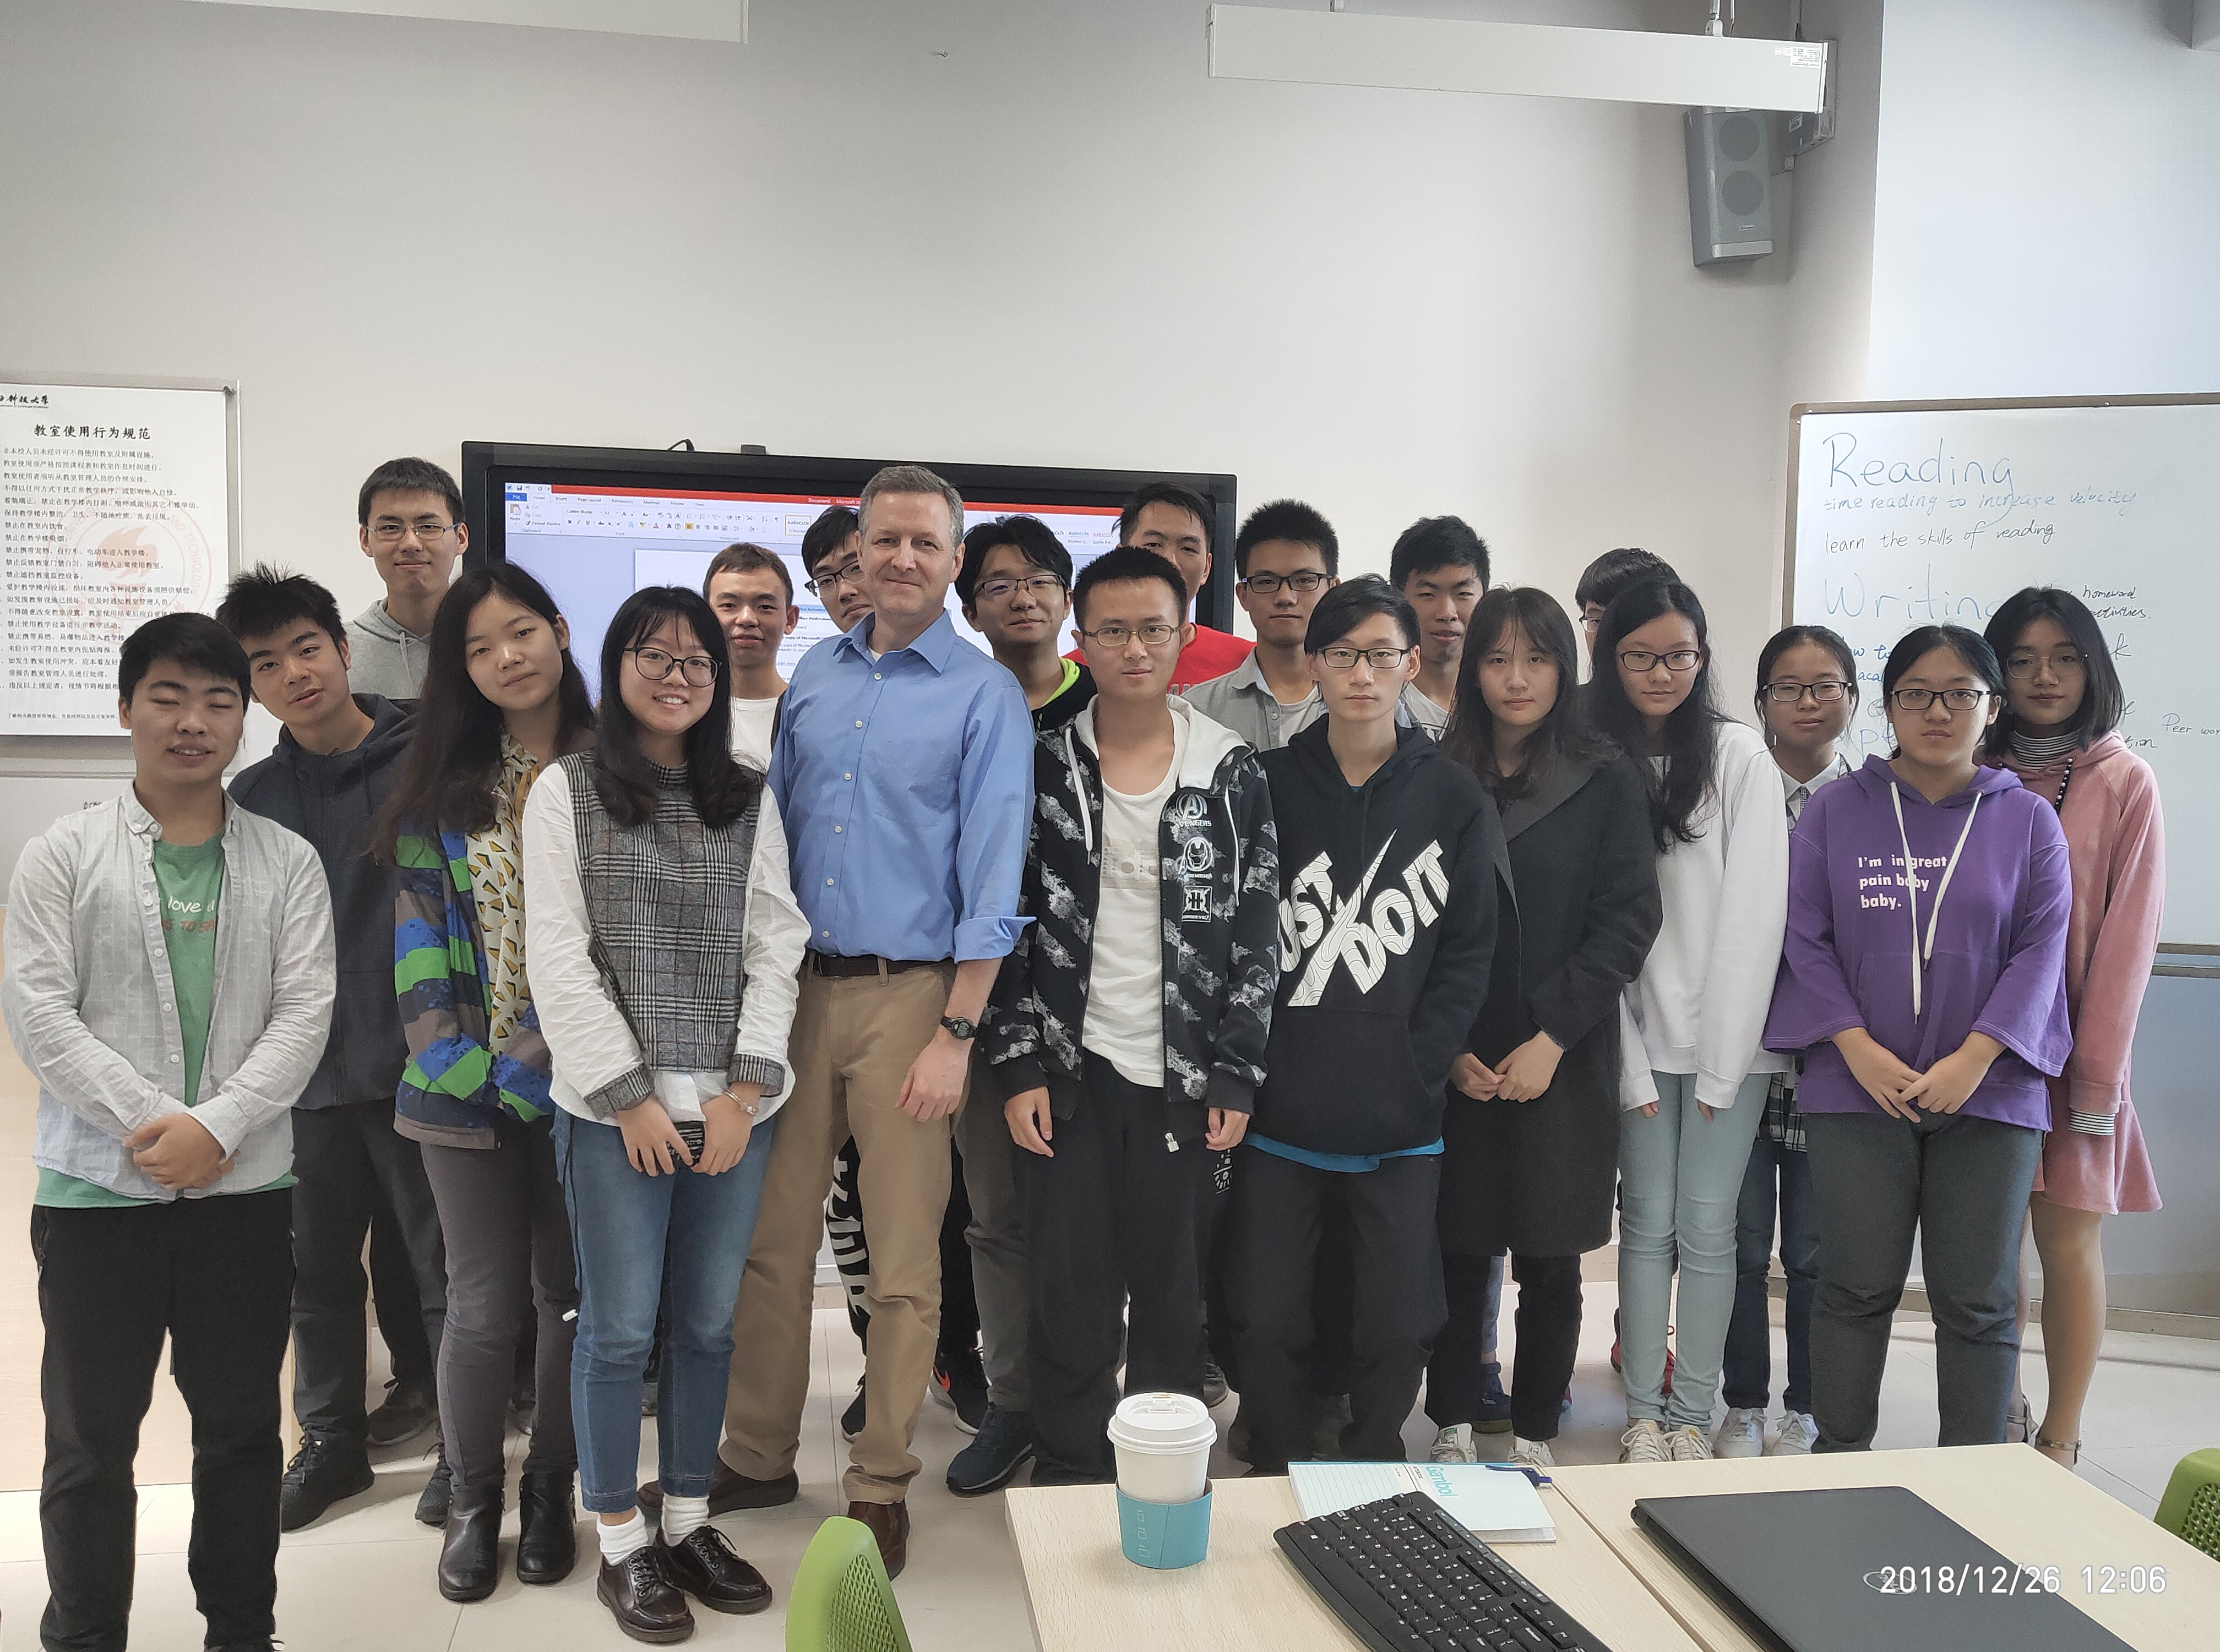
\includegraphics[height=.9\textheight]{image}
\end{center}
\clearpage

% Page 2
\begin{center}\color{BrickRed}
    \Huge Petit Papa No\"el
    \begin{vcenter}
        \begin{multicols}{2}\huge
        C'est la belle nuit de Noël\par
        La neige étend son manteau blanc\par
        Et les yeux levés vers le ciel\par
        À genoux, petits enfants\par
        Avant de fermer les paupières\par
        Font une dernière prière\par
        Petit papa Noël\par
        Quand tu descendras du ciel\par
        Avec des jouets par milliers\par
        N'oublie pas mon petit soulier\par
        Mais avant de partir\par
        Il faudra bien te couvrir\par
        Dehors tu vas avoir si froid\par
        C'est un peu à cause de moi.\par
        Il me tarde tant que le jour se lève\par
        Pour voir si tu m'as apporté\par
        Tous les beaux joujoux que je vois en rêve\par
        Et que je t'ai commandés\par
        Petit papa Noël\par
        Quand tu descendras du ciel\par
        Avec des jouets par milliers\par
        N'oublie pas mon petit soulier\par
        Et quand tu seras sur ton beau nuage\par
        Viens d'abord sur notre maison\par
        Je n'ai pas été tous les jours très sage\par
        Mais j'en demande pardon\par
        Petit papa Noël\par
        Quand tu descendras du ciel\par
        Avec des jouets par milliers\par
        N'oublie pas mon petit soulier\par
        Petit papa Noël
        \end{multicols}
    \end{vcenter}
\end{center}
\clearpage

% Page 3
\end{document}
